%  Beamer slide example.

\documentclass[9pt]{beamer}
\usepackage[utf8]{inputenc}
\usetheme{inria}
\usepackage{helvet}
\usepackage{graphicx}

\author{Maurice Bremond \and Gaëtan Harter}

\title[Intégration continue]{L'Intégration Continue}
% \subtitle{Dans un contexte de développement Inria}
\subtitle{Présentation IJD}



% Automatically insert a "new section" page at each section.
\AtBeginSection[]{
  \begin{frame}[plain]
    \partpage
  \end{frame}
}
% \inriaswitchcolors COLOR
%
% Where COLOR is one of red, blue, orange, darkblue, violet,
% pastelgreen, grey, or green.
\newcommand{\inriaswitchcolors}[1]{%
\pgfaliasimage{figfootline}{figfootline-#1}% !!!
\pgfaliasimage{figbackground}{figbackground-#1}% !!!
\pgfaliasimage{figbackground}{figbackground-#1}% !!!
}
% starting the document
% *********************
\begin{document}
% titlepage
% ---------
\begin{frame}[plain]
\titlepage
\end{frame}
% table of contents
% -----------------
\begin{frame}{\textcolor{inriaGrey}{Table des matières}}
  \tableofcontents
\end{frame}



% Introduction
% ************

\inriaswitchcolors{red}
\section{Quid de l'intégration continue}

\subsection{Qu'est-ce que c'est}
\begin{frame}{Qu'est-ce que c'est}

Contenu

\end{frame}



% L'intégration continue à Inria
% ******************************
\inriaswitchcolors{blue}
\section{L'intégration continue à Inria}




% Retour d'expérience
% *******************
\inriaswitchcolors{green}
\section{Un retour d'expérience}
\frame{\tableofcontents[currentsection]}

\subsection{Contexte de développement}

% \begin{frame}{Contexte de développement}{Plateforme de réseau de capteurs: Fit IOT-LAB}
\begin{frame}{Contexte de développement}
        Plateforme de réseau de capteurs: Fit IOT-LAB
        \begin{itemize}
                \item <2->{Réservation et utilisation de matériel réseau sans fil}
                \item <2->{Déploiement à large échelle, 3000 nœuds capteurs}
                \item <2->{Utilisé par des chercheurs depuis leur bureau}
                \item <2->{Projet d'une durée de 10ans}
        \end{itemize}
\end{frame}
\begin{frame}{Plateforme de réseau de capteurs: Fit IOT-LAB}

        IMAGE DE LA PLATEFORME COMPLETE

        Logiciels pour gérer la réservation, le déploiement et la configuration de ce matériel.



        Développement Python et C sur un linux embarqué, qui interagi avec des microcontrolleurs par port série.
        Multithread, multiprocess, communication avec un OS embarqué sur un $\mu C$.




\end{frame}

\subsection{Outils mis en place}
\frame{\tableofcontents[currentsubsection,sectionstyle=show/shaded]}

\subsubsection{Présentation des outils}
\begin{frame}{Outils mis en place}

Gestionnaire de versions: \texttt{git}
\begin{tabular}{ l | l l l }
Language         & \texttt{Python}     & \texttt{C}    & Jenkins \\ \hline
Script de build  & \texttt{setuptools} & \texttt{Make} & Bash shell, \texttt{EnvInject}\\
Compilation      & ~                   & \texttt{gcc}  & \texttt{virtualenv} \\
Tests            & \texttt{unittest}, \texttt{mock}, \texttt{nose}
                                       & \texttt{gtest} \texttt{(C++)}
                                                       & Junit, Chuck Norris\\
Couverture       & \texttt{nose-xcover}
                                   & \texttt{gcov}, \texttt{gcovr}
                                                       & Cobertura \\
Qualité de code  & \texttt{pylint}, \texttt{pep8} & ~  & Violations \\
\\
Lignes de code   &  $3000$        &  $1500$  &  $0$  \\
Lignes de tests  &  $1600 + 400$  &  $1300$  &  $0$  \\
% 1600 tests U + 400 tests intégration
Lignes de build  &  $300$         &  $170$   &  $50$ \\

% (SQLite 3.8 == 1084 * plus de tests que de code 84k source (hors blank et commentaires))
\end{tabular}
\end{frame}



\subsubsection{Jenkins}
\begin{frame}{Présentation outils}{Jenkins}
        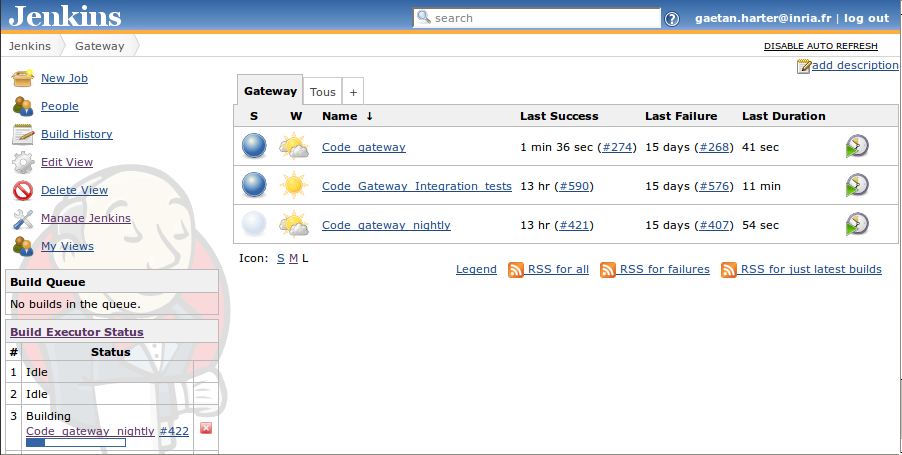
\includegraphics[width=\linewidth]{images/jenkins}
\end{frame}


\begin{frame}{Chuck Norris}{Jenkins}
% Le plus important des plugins
\begin{center}
\begin{tabular}{ l |l }
        Build KO & Build OK \\ \hline
        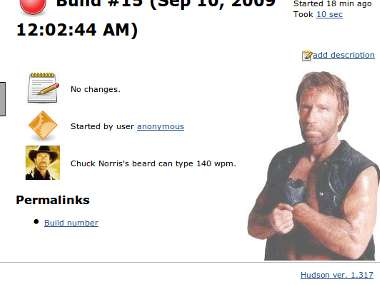
\includegraphics[height=4cm]{images/chuck_full} &
        
\includegraphics[height=4cm]{images/chuck_happy}
        %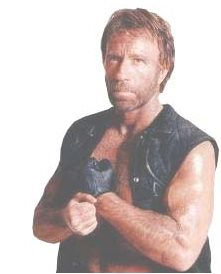
\includegraphics[height=4cm]{images/chuck_angry}
        \\
\end{tabular}
\end{center}
Chuck Norris Facts:
\begin{itemize}
  \item Chuck Norris can unit test an entire application with a single assert.
  \item Chuck Norris can divide by zero.
  \item ...
\end{itemize}
\end{frame}

\begin{frame}{Cobertura}{Jenkins}
        % Pour moi, l'outil le plus important (après chuck norris forcément)
        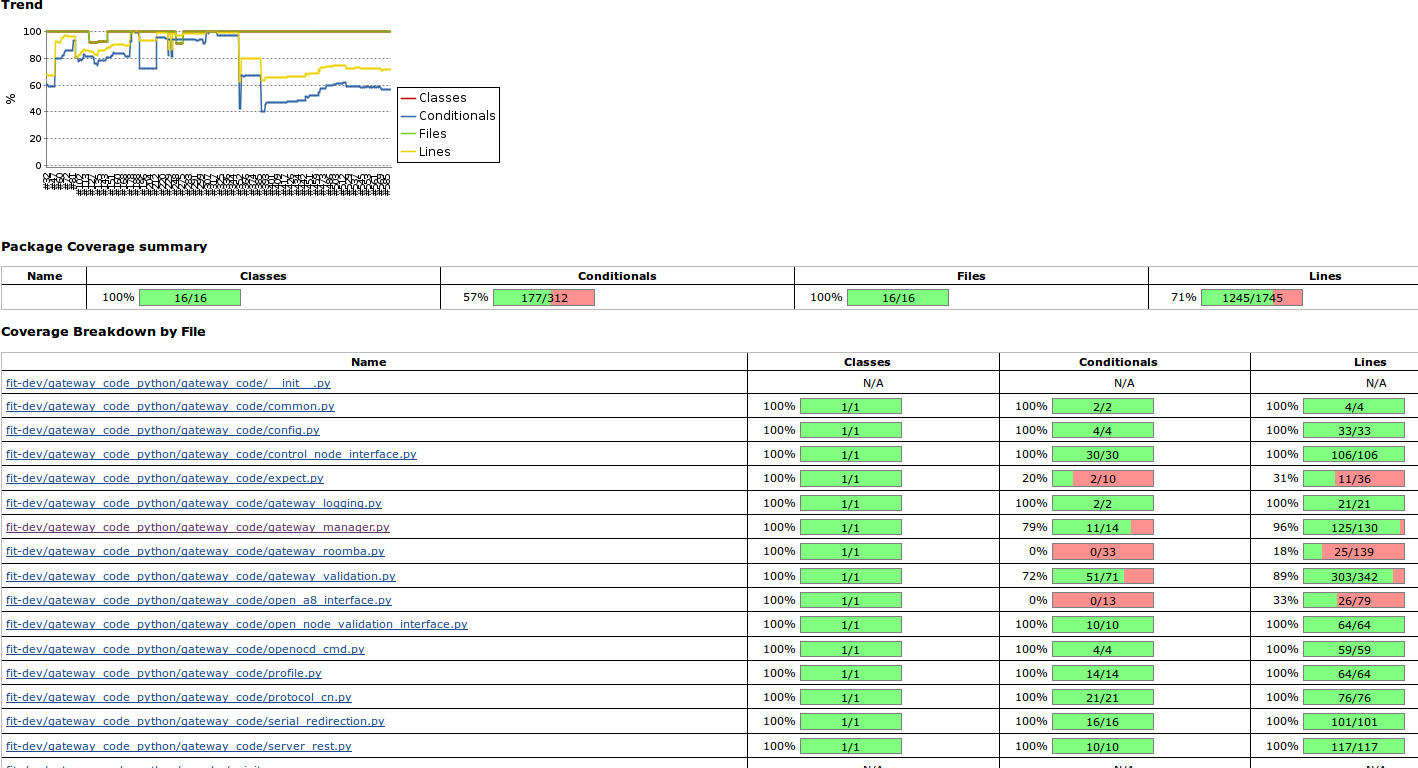
\includegraphics[width=\linewidth]{images/cobertura}\\
\end{frame}
\begin{frame}{Junit - Violations}{Jenkins}
\begin{center}
        % Juste pour montrer
        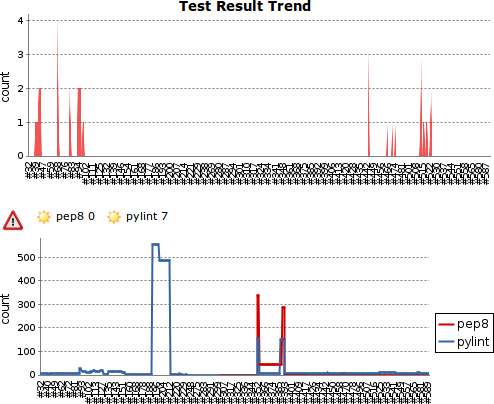
\includegraphics[height=0.8\textheight]{images/junit_violations}\\
\end{center}
\end{frame}



\subsection{Bilan}
\frame{\tableofcontents[currentsubsection,sectionstyle=show/shaded,subsubsectionstyle=show/shaded]}
\begin{frame}{Bilan}
\end{frame}

\end{document}
